
\chapter {Theoretical Background}
\label{ch:TheoreticalBackground}

This chapter provides the theoretical foundation for the key concepts relevant to the design and implementation of this project. It focuses on topics related to Large Language Models (LLMs) and the architectural characteristics of Apple Silicon (M1/M2). The sections that follow explore essential components of LLM inference, the unique hardware features of Apple Silicon, and optimizations leveraged to enable efficient on-device performance.

%----------------------
\section{Large Language Models and Inference Components}
\label{sec:LargeLanguageModelsAndInferenceComponents} 
%----------------------

Large Language Models (LLMs) are transformer-based neural networks trained on massive text corpora to generate text in human language. They can mimic human-like conversations, storytelling, and can respond to abstract instructions. These models, such as GPT, LLaMA, and Falcon, rely on the transformer architecture introduced by Vaswani et al.~\cite{vaswani2017attention}, where self-attention mechanisms enable the model to capture dependencies across different parts of the input sequence (as seen in Figure ~\ref{fig:transformer_architecture}). Inference in LLMs involves several critical components, each contributing to performance, quality, and resource efficiency.

\begin{figure}[h]
    \centering
    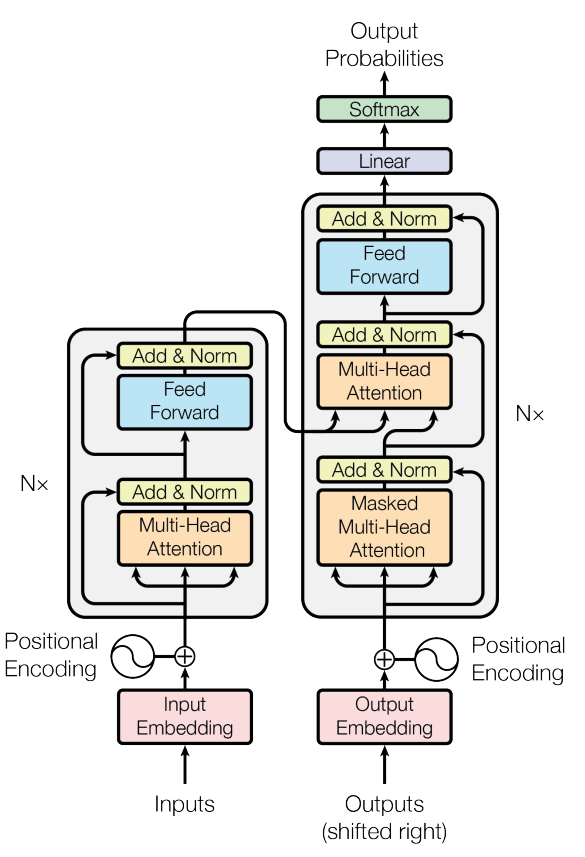
\includegraphics[width=0.4\linewidth]{images/transformer-architecture.png}
    \caption{Transformer architecture ~\cite{vaswani2017attention}}
    \label{fig:transformer_architecture}
\end{figure}
At the core of LLM inference lies the \textbf{context window}, which denotes the maximum number of tokens the model can attend to at any given time. A token is a piece of input, ranging from a subword to even a phrase, depending on the tokenization scheme of the model. For models like LLaMA-2, the context window can be up to 4,096 or 8,192 tokens~\cite{touvron2023llama}. During inference, the model builds an internal representation of this input context, which is used to generate predictions for the next token.

\begin{figure}[h]
    \centering
    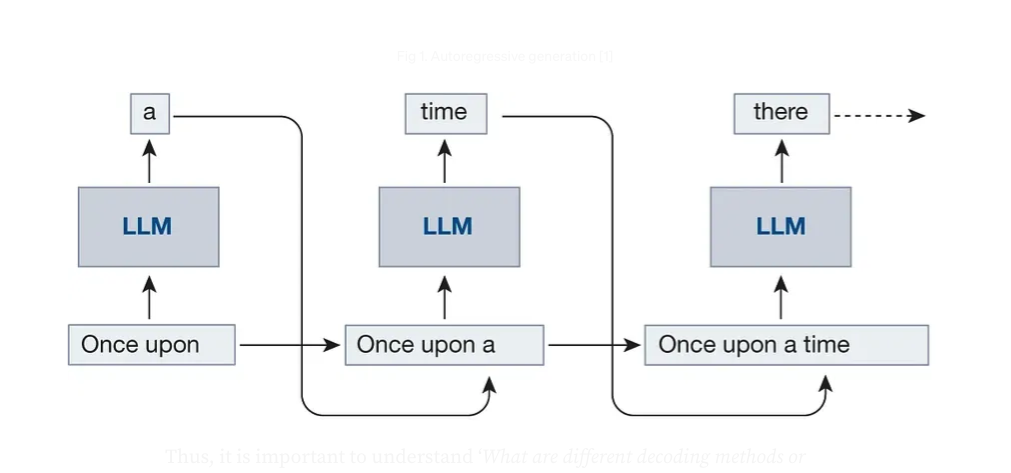
\includegraphics[width=0.6\linewidth]{images/autoregressive-decoding.png}
    \caption{Autoregressive decoding ~\cite{nabi2024all}}
    \label{fig:autoregressive_decoding}
\end{figure}

The \textbf{Key-Value (KV) cache} is a performance optimization central to LLM performance. During autoregressive decoding for text generation, a Large Language Model (LLM) processes the entire input sequence to generate a single output token. This newly generated token is then appended to the sequence, and the model repeats the process iteratively (as seen in Figure ~\ref{fig:autoregressive_decoding}). However, this leads to redundant computation over previously processed tokens at each step. To mitigate this inefficiency, the \textit{key} and \textit{value} vectors computed during the attention mechanism of the transformer can be cached. This \textit{KV caching} technique significantly reduces repeated computation by reusing the stored attention states from prior steps, thereby improving inference speed and memory efficiency. These cached representations allow the model to efficiently attend to all previously generated tokens without recalculating the entire attention graph ~\cite{alammar2018illustrated}. This caching mechanism reduces computational overhead and is especially vital when running LLMs on resource-constrained devices.

Furthermore, the token generation is governed by a sampling algorithm, which yields the output token by sampling on the output probability distribution obtained from the model. Common strategies include greedy sampling, top-$k$ sampling and temperature scaling. A \textbf{token sampler} module is responsible for leveraging these strategies to generate the output token. This can be a resource-hungry step, since this involves processing the probability distribution over the entire vocabulary of the model.

Therefore, the core components required for consistent text generation in an LLM-based system include the model weights, the LLM context (comprising the KV cache and vocabulary), and the token sampler.

Finally, the inference engine managing the model (e.g., llama.cpp, Hugging Face Transformers, or Apple CoreML) orchestrates the context construction, efficient memory handling of the KV cache, and optimized computation for each transformer layer, accounting for quantization if any. These components together define the responsiveness, accuracy, and resource efficiency of the LLM in real-time applications.

%----------------------
\section{LLM Weight Quantization}
\label{sec:LLMWeightQuantization} 
%----------------------
Quantization is a model weight compression technique that reduces the precision of the numbers used for representing model parameters. Typically, reducing the precision from 32-bit floating point to lower-bit integers such as 8-bit, 4-bit, or even 3-bit values. This significantly decreases memory usage and computational requirements, making it possible to run large language models (LLMs) efficiently on edge devices or in real-time environments without sacrificing too much accuracy \cite{jacob2017quantization,hubara2016quantized}.

Within the \texttt{ggml} framework and its application in \texttt{llama.cpp} \cite{llamacpp2023}, various quantization schemes have been introduced to significantly reduce the size and memory footprint of LLM weights. One such scheme is \texttt{Q3\_K\_L}, a 3-bit quantization format specifically designed to balance compression efficiency and model performance \cite{talamdupula2024guide,li2024quantization}. In \texttt{Q3\_K\_L}, weights are grouped in sets of 256 and quantized with shared scaling factors, offset by a zero-point, enabling fine-grained approximation while preserving hardware efficiency. Notably, \texttt{Q3\_K\_L} makes use of 4-bit storage for each quantized value (3 bits for the quantized magnitude and 1 extra bit for improved alignment and bit-packing efficiency), along with 8-bit scales and 6-bit zero-points per group. This layout ensures better alignment with SIMD instructions and allows for faster matrix-vector multiplications, which are critical during transformer inference \cite{pope2022efficiently}. ~\ref{tab:quantization-comparison} shows the comparison between common quantization schemes used in GGML. While this format slightly increases decoding complexity compared to simpler formats like \texttt{Q4\_0}, it provides a favorable tradeoff between model accuracy and size, especially for models deployed in edge or offline settings \cite{ollama2023,llamafile2023}.
Therefore, this project primarily employs model weights quantized using the \texttt{Q3\_K\_L} scheme.

\begin{table}[h]
\centering
\caption{Comparison of Common Quantization Formats in \texttt{ggml}/\texttt{llama.cpp}}
\label{tab:quantization-comparison}
\begin{tabular}{|l|c|c|c|c|}
\hline
\textbf{Format} & \textbf{Bits/Weight} & \textbf{Group Size} & \textbf{Remarks} \\ \hline
Q4\_0     & 4 bits   & 32 weights          & Baseline 4-bit scheme \\ \hline
Q4\_K     & 4 bits   & 64 weights    & Better accuracy than Q4\_0 \\ \hline
Q5\_K     & 5 bits   & 64 weights           & Higher accuracy, more storage \\ \hline
Q8\_0     & 8 bits   & 1 weight                          & No compression, baseline FP8 \\ \hline
\textbf{Q3\_K\_L}  & 3.5 bits avg & 256 weights  & High compression, optimized for SIMD \\ \hline
\end{tabular}
\end{table}


%----------------------
\section{Apple M1 System-on-Chip (SoC)}
\label{sec:AppleM1System-on-Chip} 
%----------------------

The Apple M1 chip, introduced in 2020, is a System-on-Chip (SoC) built on the ARM architecture, which integrates the CPU, GPU, and Neural Processing Unit (NPU) on a single die~\cite{apple2020m1}. This architectural design provides several advantages that are particularly relevant for local inference with large language models (LLMs), particularly for tasks like summarization and question answering.

\begin{figure}[h]
    \centering
    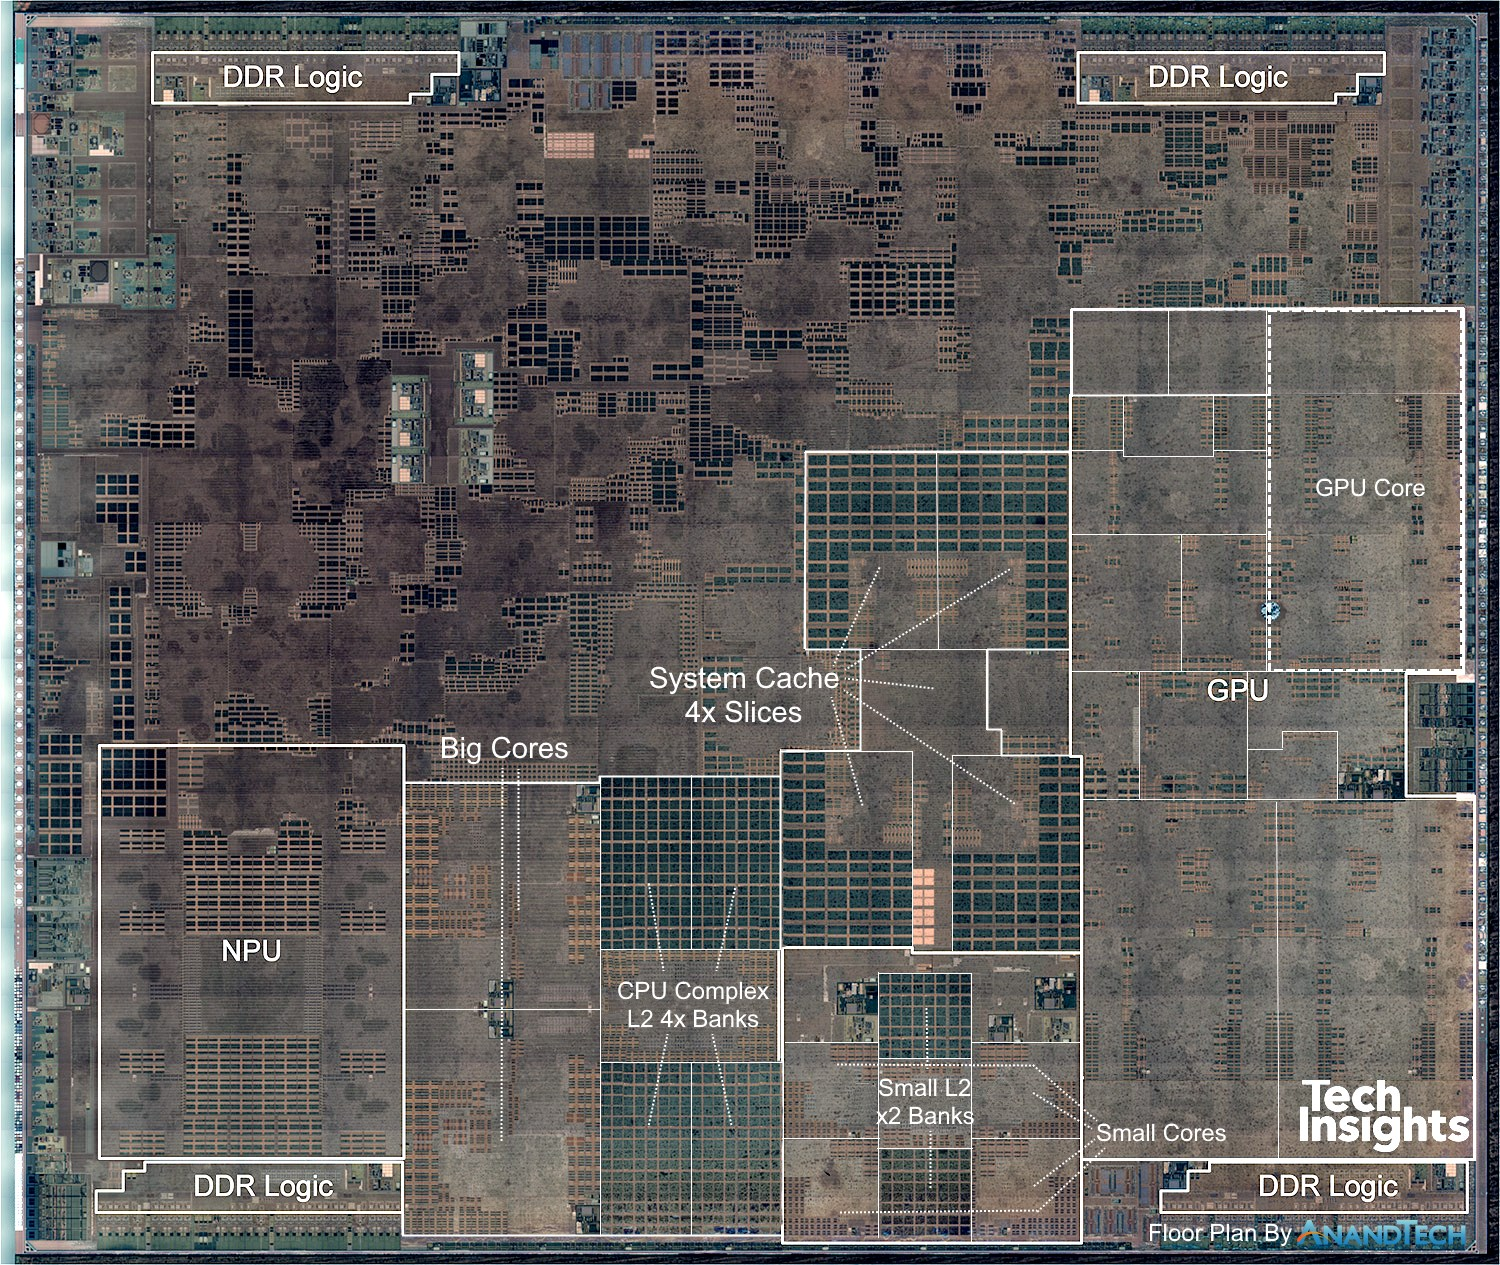
\includegraphics[width=0.8\linewidth]{images/AppleM1SOC.jpeg}
    \caption{ Apple M1 Architecture - (A12 Bionic) Chip floor plan~\cite{hollemans2020apple}}
    \label{fig:autoregressive_decoding}
\end{figure}

\subsubsection*{Unified Memory Architecture}
One of the defining features of the M1 SoC is its Unified Memory Architecture (UMA), which allows the CPU, GPU, and NPU to share the same memory pool \cite{hollemans2020apple}. This eliminates the need for memory copying across processing units and enables zero-copy execution. As a result, applications like retrieval-augmented generation (RAG) benefit from significantly reduced memory overhead and latency. Shared virtual addressing also simplifies software development by allowing seamless access to data structures across different compute units.

\subsubsection*{On-chip Accelerators: GPU and NPU}
The M1 chip includes a built-in GPU with 7--8 cores, capable of delivering up to 5.2 TOPS of performance in INT8 precision \cite{apple2020metal}. It supports general-purpose computation via Metal Shading Language (MSL), analogous to NVIDIA's CUDA, with added features like managed thread indexing and access to 7+ GB of RAM.

The Apple Neural Engine (ANE), or NPU, is an application-specific integrated circuit (ASIC) designed for efficient neural network operations. It offers 11 TOPS of INT8 compute and is exclusively used for machine learning tasks. However, it is only accessible via Apple’s CoreML framework, which supports Swift and Python interfaces. The NPU dynamically collaborates with the CPU, handling SIMD operations like matrix multiplication while delegating sequential logic to the CPU \cite{tinygrad2023apple}.

Unlike the GPU, the NPU is rarely used by general-purpose applications. This makes it a promising candidate for dedicated LLM inference workloads, as its usage is unlikely to interfere with the system's overall responsiveness.

\subsubsection*{Implications for Local LLM Inference}
The M1's integrated architecture is highly beneficial for deploying LLMs locally. Unified memory minimizes data movement, while the GPU and NPU offer parallel computation for matrix-heavy operations common in transformers. Although the NPU cannot be directly accessed via C++ (barring experimental reverse engineering efforts \cite{tinygrad2023apple}), its performance can be leveraged through CoreML model conversion pipelines \cite{apple2024coremlconvert}.

In the context of this project, these capabilities enable a lightweight, resource-efficient desktop application that performs real-time summarization and question answering over a user-provided corpus without relying on cloud resources.

